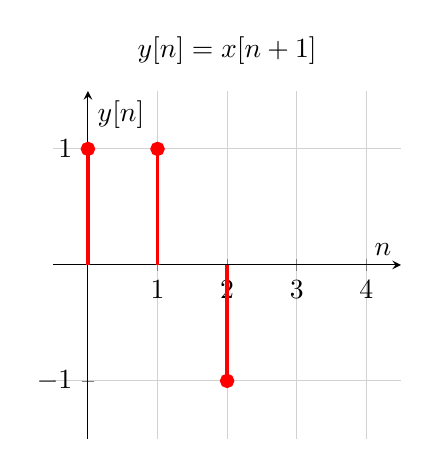
\begin{tikzpicture}
\begin{axis}[
    width=6cm,
    height=6cm,
    axis lines=middle,
    xlabel={$n$},
    ylabel={$y[n]$},
    title={$y[n] = x[n+1]$},
    xmin=-0.5, xmax=4.5,
    ymin=-1.5, ymax=1.5,
    xtick={0, 1, 2, 3, 4},
    ytick={-1, 1},
    grid=both,
    grid style={gray!15},
    major grid style={gray!35},
]

% Plot the advanced discrete-time signal
\addplot[ycomb, red, very thick, mark=*, mark size=2pt] coordinates {(0,1) (1,1) (2,-1)};

\end{axis}
\end{tikzpicture}

